\documentclass[]{aa}

\usepackage{natbib}
\usepackage{breqn}
\usepackage{xcolor}
%\bibpunct{(}{)}{;}{a}{}{,}
\usepackage{graphicx}
%\usepackage{revsymb}   
%\usepackage{amsmath}   
%\usepackage[usenames]{color}   
%\usepackage{epstopdf}  
%\DeclareGraphicsRule{.tif}{png}{.png}{`convert #1 `basename #1 .tif`.png} 
\usepackage{txfonts}
%\usepackage{amssymb}
%\usepackage{color}
%\usepackage[justification=centering]{caption}
%\bibliographystyle{aa} 
\usepackage{multirow}
%\usepackage{calrsfs}
%\usepackage[utf8]{inputenc}
%\usepackage[english]{babel}
%\usepackage{geometry} 
%\usepackage[parfill]{parskip} 
%\usepackage{amssymb}
%\usepackage{slantsc}
%\usepackage{array}
%\usepackage{url}
%\usepackage{amsmath}
%\usepackage{amsfonts}
%\usepackage[colorlinks=true,linkcolor=black, urlcolor=black, citecolor=black]{hyperref}
\usepackage{hyperref} 
%\usepackage{float}
%\usepackage{sidecap}
%\usepackage{graphicx}
%\usepackage{xcolor}
%\usepackage{epstopdf}
%\usepackage{nicefrac}
%\usepackage{subfigure}
%\usepackage{epsfig}
%\colorlet{rouge}{red!70!darkgray}
%\titlerunning{Internal rotation of Kepler 56}
%\usepackage{dutchcal}
%\usepackage[dvipsnames]{xcolor}
%\usepackage{dutchcal}
%\usepackage{cancel}
\hypersetup{
    colorlinks = true,
    linkbordercolor = {cyan},
    linkcolor={blue},
    citecolor={blue},}


\begin{document}



\def\figureautorefname{Fig.}
\def\equationautorefname~#1\null{Eq. (#1)\null}

\def\sectionautorefname{Sect.}
\def\subsectionautorefname{Sect.}
\def\subsubsectionautorefname{Sect.}


\title{SISMO: Split Inhomogeneous Solver for Modelling Oscillations}

\author{L. Fellay\inst{1} \and M.-A. Dupret\inst{1} \and  V. Antoci\inst{2}}

\institute{STAR Institute, University of Liège, 19C Allée du 6 Août, B$-$4000 Liège, Belgium \and  DTU}

\date{\today}

\abstract
% context
{Oscillation codes that solve the full fourth-order adiabatic problem couple
the mechanical variables and the perturbed gravitational potential inside a
single operator.  A \emph{split} (inhomogeneous) treatment, in which the
potential perturbation is computed independently from the current mechanical
eigenfunction and injected as a frozen source term, keeps the operator purely
mechanical.  Such an architecture is attractive as a testbed: additional
physics (for instance the Coriolis force) can later be introduced as further
source terms without modifying the operator.}
% aims
{We describe a complete reformulation of the split-Poisson method in which the
mechanical problem is reduced to a single scalar second-order equation, modes
are located and labelled by a Sturm-type determinant-sign scan without
mode-by-mode asymptotic seeding, and the well-known inaccuracy of split schemes for dipole
modes is removed by a parameter-free closure based on Takata's first
integral.}
% methods
{The two mechanical equations of the scaled adiabatic system are reduced
exactly to one second-order equation, discretised by a cell-wise exponentially
fitted staggered box scheme that yields a symmetrizable scalar tridiagonal
matrix.  The complete Cowling spectrum is obtained from the parity of a
Sturm sequence corrected for the apparent (Lamb-crossing) singularities of the
reduction.  Each mode is then refined with the frozen-potential source
recomputed at every step from an independent Poisson boundary-value problem.
For $\ell=1$ the single free amplitude of that boundary-value problem is fixed
by least-squares enforcement of Takata's first integral rather than by the
surface matching condition.}
% results
{On a $1.5\,M_\odot$ main-sequence benchmark ($25\,000$-point model,
$\ell=1,2$, $|n|=1\dots100$), the frequencies agree with the fully coupled
reference code OSC, run on the identical model, to a median of
$2\times10^{-5}$ relative, with a maximum difference of $2.1\times10^{-3}$
over all 198 modes, including the f~mode; agreement with GYRE is at the level
set by the model re-interpolation ($\simeq2\times10^{-3}$).  The complete
two-degree spectrum is obtained in $1.7\,$s on 18 threads, about forty times
faster than the coupled reference on the same model.}
% conclusions
{The gravitational potential can be treated fully inhomogeneously at the
accuracy of coupled solvers, provided (i) modes are located on the true
resonance structure of the operator rather than by mode-by-mode asymptotic estimates, and
(ii) the dipole potential is closed by momentum conservation.  The
architecture is ready for the introduction of rotational source terms.}

\keywords{asteroseismology -- stars: oscillations -- methods: numerical}

\maketitle

%=============================================================================
\section{Introduction}
\label{sec:intro}

The computation of linear adiabatic oscillations in a spherically symmetric star is conventionally formulated as a fourth-order eigenvalue problem. The governing system consists of two mechanical equations, the radial motion equation and an equation combining horizontal momentum conservation, mass conservation, and the adiabatic relation, coupled to Poisson's equation for the Eulerian perturbation of the gravitational potential, $\Phi'$ \citep[e.g.][]{unno1989}. Standard stellar oscillation codes, such as OSC \citep{scuflaire2008}, ADIPLS \citep{jcd2008}, and GYRE \citep{townsend2013}, solve these four equations simultaneously as a single coupled system.
\\~\\In the context of binary systems and tidally excited oscillations, however, we showed in \citet{Fellay2025,Fellay2026} that retaining Poisson's equation within the coupled system becomes problematic when additional physical effects and mode coupling are included. To overcome this limitation, we developed an iterative approach in which Poisson's equation is solved separately while the mechanical eigenfunctions are held fixed. The resulting gravitational-potential perturbation and its derivative are then introduced as inhomogeneous source terms in the matrix equation governing the mechanical variables and the mechanical code core is solved again.
\\~\\Although tidally excited oscillations provide a useful test case for this approach, the same formulation also offers substantial computational advantages for free stellar oscillations. By removing Poisson's equation from the coupled differential system, the discretised mechanical problem can be expressed in terms of a tridiagonal matrix rather than a $4\times4$ block matrix. This reduction decreases the cost of each matrix factorisation by approximately one order of magnitude. More importantly, the resulting inhomogeneous formulation is readily extensible. Additional physical mechanisms acting on the mechanical variables, most notably the Coriolis acceleration in a rotating star, can be included as source terms evaluated from the current eigenfunction, without requiring the underlying mechanical operator to be reconstructed. The split-Poisson formulation therefore provides a natural framework for such extensions, provided that it can first be demonstrated to reproduce the fully coupled problem with the same level of accuracy.
\\~\\Achieving this accuracy is not straightforward. Separating Poisson's equation modifies the numerical structure of the standard oscillation problem and requires the formulation of dedicated discretisation, mode-identification, and iterative-refinement procedures for both the eigenfrequencies and eigenfunctions. In this work, we present a new open-source adiabatic stellar oscillation code, SISMO (Split Inhomogeneous Solver for Modelling Oscillations), based on a split treatment of Poisson's equation, in which the effects not included in the mechanical operator are introduced through inhomogeneous terms. 
\\~\\In \autoref{sec:formulation}, we introduce the principle behind the classical adiabatic oscillation problem, describe our new idea to solve it, and introduce the basic mathematical formalism and variables used in SISMO. Then in \autoref{sec:core} we present the core solver of the code, the discretisation and boundary conditions that are imposed in the code. In \autoref{sec:sturm}, we present the mode finding method and the convergence method used to converge toward the eigenfunctions and eigenvalues. Finally, in \autoref{sec:results}, we present benchmark against two classical adiabatic stellar oscillation codes GYRE and CLES, comparing both the frequency and computation times obtained with those codes.

%=============================================================================
\section{Overview of the method}
\label{sec:formulation}

\subsection{The problem, and the idea}
\label{sec:overview}
The linear adiabatic oscillations of a spherical star are described by four coupled first-order equations: two \emph{mechanical} equations, which govern the fluid displacement and the pressure perturbation, and the two components of Poisson's equation, which govern the perturbation of the gravitational potential $\Phi'$ and its radial derivative.  A coupled code solves all four at once.  The idea of the split method is different, we solve only the two mechanical equations, and treat the gravitational potential as a known external forcing, recomputed from the current displacement field between iterations.
\\~\\This turns the eigenvalue problem into a fixed-point problem.  Starting from an approximate eigenfunction, we (i) compute the potential perturbation that this eigenfunction generates, by solving Poisson's equation on its own; (ii) insert that potential into the mechanical equations as a fixed source term; (iii) solve the resulting forced mechanical problem and update the frequency; and (iv) repeat until the eigenfunction regenerates its own potential.  At that point the pair (frequency, eigenfunction) solves the original coupled problem exactly: nothing is neglected, the split changes how the solution is found, not what is solved.  Its interest is architectural.  The operator that must be assembled and factorised at every step contains only the mechanics, so it is small and cheap; and any additional force one wishes to study later (the Coriolis force is our
motivation) can be added as one more source term in step~(ii), without ever touching the operator.
For the case considered here, the split Poisson equation without the Coriolis force, complete calculation proceeds in two stages for each spherical degree $\ell$:
\begin{enumerate}
\item Locate the modes of the mechanical (Cowling) operator in the requested frequency window. This is done by a counting technique (Sect.~\ref{sec:sturm}): a period sweep identifies intervals with an odd change in the corrected count, and bisection locates the enclosed mode. The sampling must be fine enough to resolve adjacent modes.
\item Refine each located mode with the gravitational source switched on (Sect.~\ref{sec:refine}), using the fixed-point iteration described above.  The frequency moves from its Cowling value to the full value; the shift is below a percent for most modes and largest for low-order dipole modes, which receive a dedicated treatment (Sect.~\ref{subsec_dipole_closure}).
\end{enumerate}
The remainder of this section defines the variables and the two building blocks (the mechanical pair and the Poisson problem); the numerical core is described in Sect.~\ref{sec:core}.

\subsection{Variables and coefficients}
\label{sec:variables}

We work with the scaled variables of the OSC adiabatic system~5, which absorb the leading behaviour of the physical quantities at the centre and keep all variables of order unity.  With $x=r/R$ the fractional radius and $\sigma^2=\omega^2$ the squared frequency in units of $GM/R^3$, the stellar structure enters through five functions of $x$:
\begin{equation}
  S_2=\frac{m(x)}{x^3},\quad
  S_3=\frac{P}{\rho},\quad
  S_4=\rho,\quad
  S_5=\Gamma_1,\quad
  S_6=A_{\rm osc},
\end{equation}
where $m(x)$ is the fractional mass inside $x$.  Two combinations occur repeatedly: the local dimensionless gravity is $g=S_2x$, and, with the OSC sign convention for $A_{\rm osc}$, the squared Brunt--V\"ais\"al\"a (buoyancy) frequency is
\begin{equation}
  N^2=-S_2S_6x^2 .
\end{equation}
Thus a stably stratified g-mode cavity has $S_6<0$.  The four dependent variables are the scaled radial displacement, horizontal displacement, potential perturbation, and potential gradient:
\begin{align}
  y_1 &= \frac{\xi_r}{x^{\max(0,\ell-1)}}, &
  y_2 &= \frac{\sigma^2\,\xi_h}{x^{\max(0,\ell-1)}S_2}, \nonumber\\
  y_3 &= \frac{\Phi'}{x^{\ell}S_2}, &
  y_4 &= \frac{\partial_x\Phi'}{x^{\max(0,\ell-1)}S_2}.
  \label{eq:variables}
\end{align}
There is no separate pressure variable: the Eulerian pressure perturbation is carried by the difference $y_2-y_3$,
\begin{equation}
  \frac{P'}{P} = x^{\ell}\,\frac{S_2}{S_3}\,(y_2-y_3),
  \label{eq:pprime}
\end{equation}
a relation that follows from the horizontal momentum equation (which is algebraic in the adiabatic case) and that will be needed again for the dipole closure of Sect.~\ref{subsec_dipole_closure}. In these variables the two mechanical equations take the compact form
\begin{align}
  \frac{{\rm d}y_1}{{\rm d}x} &= a_{11}y_1+a_{12}y_2+a_{13}y_3,
  \label{eq:mech1}\\
  \frac{{\rm d}y_2}{{\rm d}x} &= a_{21}y_1+a_{22}y_2+a_{23}y_3 ,
  \label{eq:mech2}
\end{align}
with the coefficients
\begin{align}
  a_{11} &= -\frac{\ell+1}{x}+d_{13}, &
  a_{12} &= \frac{\ell(\ell+1)S_2}{x\,\sigma^2}-d_{13}, \nonumber\\
  a_{13} &= d_{13}, &
  a_{21} &= c_{21}+\frac{\sigma^2}{xS_2}, \nonumber\\
  a_{22} &= c_{33}-c_{21}, &
  a_{23} &= c_{21},
  \label{eq:coeffs}
\end{align}
where
\begin{equation}
  d_{13}=\frac{xS_2}{S_3S_5},\qquad
  c_{21}=xS_6,\qquad
  c_{33}=\frac{3-S_4/S_2-\ell}{x}.
\end{equation}
Note that the potential enters the mechanics only through $y_3$ (via $a_{13}$ and $a_{23}$); the gradient $y_4$ does not appear.  This is why, in the split scheme, only $y_3$ needs to be supplied as a source. One coefficient deserves a warning, because the point is invisible in the usual block formulation.  In the underlying OSC system the derivative of the first equation carries a weight $\sigma^2$; once the equation is divided by that weight, the off-diagonal coefficient $a_{12}$ acquires the term $\ell(\ell+1)S_2/(x\sigma^2)$.  This $1/\sigma^2$ is not a detail: it is what carries the gravity-mode physics.  A quick way to see it is to form the local radial wavenumber of the pair,
\begin{equation}
  k_r^2 \simeq -a_{12}\,a_{21}
        \simeq \frac{\ell(\ell+1)}{x^2}
          \left(\frac{N^2}{\sigma^2}-1\right),
  \label{eq:wkbcheck}
\end{equation}
which is the standard asymptotic dispersion relation of gravity modes, with its unbounded accumulation of modes as $\sigma\to0$.  An implementation that forgets the derivative weight loses the $1/\sigma^2$ and produces a spectrum with only a finite number of gravity modes -- a qualitatively wrong result that is nevertheless easy to mistake for a subtle bug. Equation~(\ref{eq:wkbcheck}) is a one-line sanity check that we recommend to anyone re-implementing the system.

\subsection{The independent Poisson problem}
\label{sec:poissonbvp}
The potential pair obeys the two remaining equations of the system,
\begin{align}
  \frac{{\rm d}y_3}{{\rm d}x} &= c_{33}\,y_3+\frac{1}{x}\,y_4,
  \label{eq:poi1}\\
  \frac{{\rm d}y_4}{{\rm d}x} &= -c_{21}\frac{S_4}{S_2}\,y_1+c_{42}\,y_2
     +\Big[\frac{\ell(\ell+1)}{x}-c_{42}\Big]y_3
     +\Big(c_{33}-\frac{1}{x}\Big)y_4,
  \label{eq:poi2}
\end{align}
with $c_{42}=xS_4/(S_3S_5)$.  These are the scaled form of $\nabla^2\Phi'=4\pi G\rho'$: the terms in $y_1$ and $y_2$ on the right-hand side of Eq.~(\ref{eq:poi2}) are the density perturbation generated by the displacement field.  In the split scheme these equations never enter the eigenvalue operator.  They define a small, self-contained boundary-value problem: given the current mechanical iterate $(y_1,y_2)$, find the potential it generates.
\\~\\The problem is linear, so its solution is built from two pieces.  A particular solution $(y_3^{\rm p},y_4^{\rm p})$ is integrated outward from the centre (fourth-order Runge--Kutta) with the $(y_1,y_2)$ source, it contains the response to the density perturbation, but does not yet satisfy the outer boundary condition.  A homogeneous solution $(y_3^{\rm h},y_4^{\rm h})$ is integrated starting from the regular central behaviour $y_4=\ell\,y_3$. The full solution is
\begin{equation}
  \begin{pmatrix}y_3^\Phi\\[2pt] y_4^\Phi\end{pmatrix}
  =\begin{pmatrix}y_3^{\rm p}\\[2pt] y_4^{\rm p}\end{pmatrix}
  + A \begin{pmatrix}y_3^{\rm h}\\[2pt] y_4^{\rm h}\end{pmatrix},
  \label{eq:phABC}
\end{equation}
where $A$ is a constant classically set by the vacuum condition at the photospheric interior--atmosphere raccord (the interior potential must match a decaying exterior solution),
\begin{equation}
  y_4+(\ell+1)\,y_3=-\frac{S_4}{S_2}\,y_1 \qquad (x=x_{\rm ph}).
  \label{eq:surfBC}
\end{equation}
\\~\\For $\ell\ge2$ this closure works well.  In a model containing an explicit atmosphere, SISMO applies it at the recorded photospheric raccord, not at the last atmospheric point; models without raccord metadata use their final point.  The homogeneous solution grows outward as $x^{\ell}$, so its residual and the particular-solution residual must be evaluated at the same point.  The dipole remains more sensitive because the resulting amplitude affects the potential throughout the star.  A small local mismatch can therefore be propagated globally.  \autoref{subsec_dipole_closure} replaces this pointwise closure for $\ell=1$ by a condition that involves the whole star.

%=============================================================================
\section{The scalar second-order core}
\label{sec:core}

\subsection{From two equations to one}
\label{sec:reduction}
Because the gravitational-potential perturbation is held fixed during each mechanical solve, Eqs.~(\ref{eq:mech1})--(\ref{eq:mech2}) form a linear system of two first-order differential equations with a prescribed source term. This system can be reduced exactly to a single second-order equation for either mechanical variable. Focussing on $y_1$, which is directly related to the displacement, and eliminate $y_2$ using Eq.~(\ref{eq:mech1}) gives:
\begin{equation}
y_2=\frac{y_1'-a_{11}y_1-a_{13}y_3}{a_{12}} .
\label{eq:y2elim}
\end{equation}
Substitution into Eq.~(\ref{eq:mech2}) yields a second-order equation of Sturm--Liouville type,
\begin{equation}
y_1''+\alpha(x)y_1'+\beta(x)y_1 = R(x),
\label{eq:secondorder}
\end{equation}
where the coefficients $\alpha$ and $\beta$ are combinations of the $a_{ij}$ and their derivatives, while the source term $R$ depends linearly on $y_3$ and its derivative. This reduction introduces no approximation. Its main advantage is numerical: discretising a scalar second-order equation on $N$ mesh points produces an $N\times N$ tridiagonal system, instead of the $4\times4$ block-banded system associated with the original formulation. The resulting linear system can therefore be factorised and solved at substantially lower computational cost.
\\~\\The reduction nevertheless introduces a division by $a_{12}$ in Eq.~(\ref{eq:y2elim}). This coefficient vanishes at the radius where $\sigma^2$ equals the local Lamb-frequency term,
\begin{equation}
\sigma^2=\frac{\ell(\ell+1)S_3S_5}{x^2}.
\end{equation}
This apparent singularity does not compromise the formulation for two reasons. First, the choice to eliminate $y_2$, rather than $y_1$, places the corresponding singular point in a comparatively benign region. For gravity modes, the Lamb-frequency crossing generally lies in the outer evanescent region, away from the main propagation cavity. Eliminating $y_1$ instead would introduce a singularity where $\sigma^2=N^2$, namely close to the turning points that delimit the propagation cavity of each g mode.
\\~\\Second, the singularity is not present in the underlying first-order system, which remains regular at the crossing. The two local solutions of Eq.~(\ref{eq:secondorder}) also remain regular. The vanishing of $a_{12}$ therefore represents a local differential constraint rather than a physical singularity. At the crossing radius, Eq.~(\ref{eq:mech1}) loses its dependence on $y_2$ and directly relates $y_1'$ to $y_1$ and to the prescribed source. A suitable discretisation must recover this constraint without requiring a special matching condition. As shown below, this property is built into the adopted numerical scheme.
%A further numerical difficulty arises when transforming Eq.~(\ref{eq:secondorder}) into self-adjoint form. The standard transformation consists of multiplying the equation by the integrating factor
%\begin{equation}
%\exp\left(\int \alpha{\rm d}x\right).
%\end{equation}
%When evaluated globally across the stellar model, however, this factor can vary by several hundred orders of magnitude. A stellar model typically spans approximately 200 pressure scale heights, and $\alpha$ additionally contains a $\sigma^2$-dependent singular contribution near the centre. The resulting dynamic range exceeds that of double-precision arithmetic and makes the direct use of a global integrating factor numerically impractical.
%The self-adjoint transformation must therefore be applied locally rather than globally, with the integrating factor evaluated separately over each grid cell. This local construction avoids the excessive dynamic range while preserving the structure required for the discretisation. The corresponding scheme is described in the following subsection.


\subsection{Discretisation on a node--face grid}
\label{sec:scheme}

Section~\ref{sec:reduction} shows that the two mechanical equations can be reduced to one second-order equation for $y_1$. In the code, we construct the discrete scalar equation directly from the original first-order pair. This avoids differentiating the stellar-model coefficients and preserves the regular behaviour of the original equations when $a_{12}$ vanishes.

We use the original stellar grid without remeshing. The displacement variable $y_1$ is stored at the model points $x_i$, called \emph{nodes}, whereas $y_2$ is stored halfway between adjacent nodes, at \emph{faces}. Around node $i$, the arrangement is
\[
\underbrace{y_{1,i-1}}_{\text{node}}
\;\longleftrightarrow\;
\underbrace{y_{2,f^-}}_{\text{face}}
\;\longleftrightarrow\;
\underbrace{y_{1,i}}_{\text{node}}
\;\longleftrightarrow\;
\underbrace{y_{2,f^+}}_{\text{face}}
\;\longleftrightarrow\;
\underbrace{y_{1,i+1}}_{\text{node}} .
\]
This placement follows the equations themselves. Equation~(\ref{eq:mech1}) describes the change of $y_1$ across one cell, so it connects two nodes through the face value of $y_2$. Equation~(\ref{eq:mech2}) describes the change of $y_2$ across the control volume around a node, so it connects the two neighbouring faces through the nodal value of $y_1$.

Within each cell, the coefficients are treated as constant and the differential equation is integrated analytically. Applying this construction to Eq.~(\ref{eq:mech1}) over the cell $[x_i,x_{i+1}]$, of width $h$, gives
\begin{equation}
y_{1,i+1}
={\rm e}^{p}y_{1,i}
+h\,\varphi_1(p)
\left(
\bar a_{12}y_{2,f}
+\bar a_{13}\bar y_3
\right),
\qquad
p=\bar a_{11}h ,
\label{eq:face_relation}
\end{equation}
where overbars denote cell averages and
\[
\varphi_1(p)=\frac{{\rm e}^{p}-1}{p},
\qquad
\varphi_1(0)=1 .
\]
The factor $\varphi_1$ makes the update exact for the piecewise-constant coefficients used in the cell. For small $p$, it tends to the usual finite-difference update. More importantly, Eq.~(\ref{eq:face_relation}) can be read simply as follows: given $y_1$ at the two nodes and the source $y_3$, it determines the value of $y_2$ at the face between them.

Applying the same construction to Eq.~(\ref{eq:mech2}) over the volume between faces $f^-$ and $f^+$, of width $V_i$, gives
\begin{equation}
y_{2,f^+}
={\rm e}^{q}y_{2,f^-}
+V_i\,\varphi_1(q)
\left(
a_{21,i}y_{1,i}+a_{23,i}y_{3,i}
\right),
\qquad
q=a_{22,i}V_i .
\label{eq:node_relation}
\end{equation}

We now eliminate the face values. Equation~(\ref{eq:face_relation}) expresses $y_{2,f^-}$ in terms of $y_{1,i-1}$ and $y_{1,i}$, and $y_{2,f^+}$ in terms of $y_{1,i}$ and $y_{1,i+1}$. Substituting these two expressions into Eq.~(\ref{eq:node_relation}) leaves one equation involving only three neighbouring values of $y_1$. Repeating this at every node gives
\begin{equation}
\mathsf{T}(\sigma^2)\,\mathbf{y}_1
=\mathbf{r}(y_3),
\end{equation}
where $\mathsf{T}$ is tridiagonal and $\mathbf{r}$ contains the prescribed gravitational source. This is the discrete scalar problem introduced in Sect.~\ref{sec:reduction}; the face variable $y_2$ is reconstructed only when it is needed.

\paragraph{The Lamb-frequency crossing.}
Solving Eq.~(\ref{eq:face_relation}) for $y_{2,f}$ introduces a factor $1/\bar a_{12}$. The coefficients therefore become large near the radius where $\bar a_{12}=0$, but the physical solution is regular there. At the crossing, Eq.~(\ref{eq:face_relation}) stops determining $y_2$ and instead imposes the constraint
\[
y_{1,i+1}
-{\rm e}^{p}y_{1,i}
-h\,\varphi_1(p)\bar a_{13}\bar y_3
=0 .
\]
The large discrete coefficients enforce this constraint automatically as the crossing is approached. Numerically, the code protects the division against an exact zero and replaces isolated, anomalously large reconstructed face values by a local average. It still needs no turning-point detection or matching condition.

\paragraph{Why this matrix can count modes.}
The matrix is not written symmetrically, but its two couplings across each active interior face have a positive product:
\begin{equation}
\mathsf{T}_{i,i+1}\,
\mathsf{T}_{i+1,i}
=
\frac{{\rm e}^{\,q_{i+1}+p_f}}
{\big(h\varphi_1\bar a_{12}\big)_f^2}
>0 .
\label{eq:posprod}
\end{equation}
Each connected interior block can therefore be rescaled into symmetric form. A boundary condition may set an end coupling to zero; this simply ends a block and does not change the counting argument. The factorisation provides Sturm sign information \citep[e.g.][]{wilkinson1965}: after correcting for the known poles at $\bar a_{12}=0$, the number of negative pivots changes whenever the trial value of $\sigma^2$ crosses an eigenvalue. Section~\ref{sec:sturm} explains how SISMO uses this property to locate modes.
\subsection{Boundary rows}
\label{sec:bc}

The system is closed by two rows representing the physical boundary conditions of the original oscillation problem, expressed in the same set of variables. At the stellar surface, the Lagrangian pressure perturbation vanishes,
$\delta P=0$. Using Eq.~(\ref{eq:pprime}), this condition reduces to
\begin{equation}
y_1-y_2+y_3=0
\qquad (x=x_{\rm s}).
\end{equation}
The surface boundary condition is combined with the half-cell form of Eq.~(\ref{eq:face_relation}) to construct the final row of the discrete system. At the centre, regularity imposes a linear relation between $y_1$ and $y_2$. For a grid extending to $x=0$, this relation may be written, for example, as
\begin{equation}
\sigma^2 y_1=\ell S_2,y_2.
\end{equation}
In practice, the condition is imposed at the first grid point satisfying $x>10^{-8}$. This avoids evaluating the formally singular $1/x$ terms in the coefficients at radii that are numerically indistinguishable from zero, without affecting the physical central boundary condition. Both boundary rows remain confined to the tridiagonal bandwidth and preserve the positive-product property given by Eq.~(\ref{eq:posprod}). The Sturm-counting structure of the discrete operator is therefore retained after the boundary conditions are imposed.
%=============================================================================
\section{Mode location and refinement}
\label{sec:sturm}

The calculation separates two different tasks:
\begin{enumerate}
\item Temporarily set the gravitational source to zero and locate the modes of the mechanical, or Cowling, problem in the requested frequency range.
\item Use each Cowling mode as the starting point for an iteration that makes the displacement and its gravitational potential mutually consistent.
\end{enumerate}
The first stage answers \emph{Where are the modes?} using only the inexpensive tridiagonal matrix. The second answers \emph{How does the gravitational source change each mode?} and is carried out only for the modes that will be retained.

\subsection{Locating the Cowling modes}

For a trial value of $\sigma^2$, SISMO factorises the tridiagonal matrix $\mathsf{T}(\sigma^2)$. Section~\ref{sec:scheme} showed that its connected blocks can be rescaled into symmetric form. Their negative pivots therefore provide a Sturm count. This is the main advantage over a mode-by-mode search: no individual starting frequency is required.

One correction is needed. The matrix contains $1/\bar a_{12}$, and the position where $\bar a_{12}=0$ moves through the grid as the trial frequency changes. When this position crosses a face, one matrix pivot changes sign even though no physical eigenvalue has been crossed. At the same time, the number of faces with $\bar a_{12}<0$ also changes by one. Adding the two counts removes this spurious event:
\begin{equation}
\mathcal{S}(\sigma^2)
=
\#\{\text{negative pivots}\}
+
\#\{\text{faces with }\bar a_{12}<0\}.
\label{eq:indicator}
\end{equation}
A Lamb-frequency pole leaves $\mathcal{S}$ unchanged, whereas a genuine eigenvalue changes it.

In practice, SISMO first chooses a frequency interval broad enough to contain the requested radial orders. The asymptotic g-mode relation is used only to set these outer limits, not to guess individual mode frequencies.  Its buoyancy integral uses $N/x=\sqrt{\max(0,-S_2S_6)}$, so convectively unstable layers do not contribute. The interval is sampled uniformly in period because high-order g modes are approximately equally spaced in period. The sampling is chosen so that adjacent trial points normally contain at most one mode. The code brackets an interval when $\mathcal{S}$ changes by an odd number; in the intended one-mode-per-interval case, this change is one. Bisection then refines the enclosed eigenfrequency to a relative precision of $10^{-12}$.

A few inverse-iteration steps then recover the eigenfunction associated with each frequency. The result of the scan is an ordered set of Cowling frequencies and eigenfunctions, including the g-mode sequence and any f and low-order p modes inside the interval. Each matrix factorisation is independent and costs $\mathcal{O}(N)$ operations, so the scan and the bisections can be distributed directly across threads.

%=============================================================================
\subsection{Refinement with the gravitational source}
\label{sec:refine}

A Cowling mode is only the starting point. In the full problem, the displacement generates a potential through Poisson's equation, while that same potential acts as a source in the mechanical equation. The solution is reached when these two statements are simultaneously true. SISMO enforces this consistency by repeating the following steps for each mode.

\begin{enumerate}
\item \emph{Update the potential.}
Starting from the current $y_1$, the code reconstructs $y_2$ and solves the independent Poisson problem of Sect.~\ref{sec:poissonbvp}. To prevent the displacement and potential from overshooting one another, the new source is mixed with the previous one:
\begin{equation}
y_3
\leftarrow
\alpha y_3^{\rm new}
+(1-\alpha)y_3^{\rm old}.
\end{equation}
The mixing factor $\alpha$ is configurable; the benchmark calculations use $\alpha=0.4$.

\item \emph{Update the mode.}
At the current frequency, one factorisation of $\mathsf{T}$ provides two response vectors,
\begin{align}
\mathbf{z}
&=
\mathsf{T}^{-1}
\left[
\mathbf{r}(y_3)-\mathsf{T}\mathbf{y}_1
\right], \nonumber\\
\mathbf{t}
&=
\mathsf{T}^{-1}\mathsf{T}'\mathbf{y}_1,
\qquad
\mathsf{T}'=
\frac{\partial\mathsf{T}}{\partial\sigma^2}.
\end{align}
Here $\mathbf{z}$ corrects the mismatch in the mechanical equation if the frequency is held fixed, while $\mathbf{t}$ measures how the solution responds to a change in frequency. The derivative $\mathsf{T}'$ is obtained by a finite difference.

Projecting these two responses onto the current eigenfunction gives the Newton frequency correction
\begin{equation}
\delta\sigma^2
=
\frac{\langle\mathbf{y}_1,\mathbf{z}\rangle}
     {\langle\mathbf{y}_1,\mathbf{t}\rangle}.
\end{equation}
The frequency and eigenfunction are then updated together:
\begin{equation}
\sigma^2
\leftarrow
\sigma^2+\delta\sigma^2,
\qquad
\mathbf{y}_1
\leftarrow
\mathbf{y}_1+\mathbf{z}-\delta\sigma^2\mathbf{t}.
\end{equation}
The frequency step is limited to $10^{-3}\sigma^2$ so that the iteration cannot jump to a neighbouring mode. The eigenfunction is normalised after each update. Its sign is also aligned with the preceding iterate; otherwise the arbitrary sign of an eigenfunction can make the displacement and potential alternate between two equivalent states.

\item \emph{Test convergence.}
The iteration stops when the unconstrained relative frequency correction is below $\max(10^{-7},\epsilon_{\rm tol})$, where $\epsilon_{\rm tol}$ is the requested tolerance, and the potential has stabilised. If the maximum number of iterations is reached, SISMO returns the iterate with the smallest unconstrained frequency correction rather than simply returning the last one. This best-iterate rule is useful when a small residual cycle remains.
\end{enumerate}

Modes are refined independently, so this stage is parallelised over modes.

%=============================================================================
\subsection{The dipole closure}
\label{subsec_dipole_closure}

The Poisson solution is the sum of a particular solution and a homogeneous solution with one free amplitude $A$ [Eq.~(\ref{eq:phABC})]. For $\ell\geq2$, the surface vacuum condition determines $A$ accurately. The dipole case, $\ell=1$, is more sensitive: the homogeneous solution grows outwards, so a small error where the surface condition is applied can affect the potential throughout the star and noticeably shift the frequency.

For dipole modes, momentum conservation supplies a more robust condition. A uniform translation of the whole star is a zero-frequency solution, and the dipole equations therefore possess the first integral derived by \citet{takata2005,takata2006}. Defining
\begin{equation}
\phi=xS_2y_3,
\qquad
\partial_x\phi=S_2y_4,
\end{equation}
and writing $a=\xi_r$ and $\bar p$ for the scaled pressure perturbation, the integral is
\begin{equation}
J(x)
=
\sigma^2x\rho\,a
-P\bar p
-(\sigma^2+2S_2)\phi
+x(\sigma^2-S_2)\partial_x\phi
=0 .
\label{eq:takata}
\end{equation}
For an exact dipole mode, $J$ vanishes at every radius.

The important simplification is that $J$ depends linearly on the free amplitude $A$. At grid point $i$, we can write
\begin{equation}
J_i(A)=M_i+A H_i,
\end{equation}
where $M_i=J_i(0)$ is the value obtained from the particular solution and $H_i=J_i(1)-J_i(0)$ is the change produced by one unit of the homogeneous solution. These definitions contain the same information as the explicit expansion into particular and homogeneous terms, but make the role of $A$ clearer.

During an intermediate iteration, the mechanical and gravitational variables are not yet fully consistent, so no single value of $A$ generally makes every $J_i$ exactly zero. Instead, SISMO chooses the value that minimises the residual over the whole star,
\begin{equation}
\sum_i w_i\,|M_i+A H_i|^2,
\end{equation}
where $w_i$ are trapezoidal integration weights. The minimum is obtained directly:
\begin{equation}
A
=
-\frac{\displaystyle\sum_i w_i H_i^{*}M_i}
       {\displaystyle\sum_i w_i |H_i|^2}.
\label{eq:closure}
\end{equation}

This global closure lets all interior grid points contribute to the choice of $A$, instead of relying on one value at the surface. It requires only two weighted scalar products, introduces no adjustable parameter, and leaves the mechanical operator unchanged. Section~\ref{sec:results} shows that it brings the dipole modes close to the accuracy obtained for the quadrupole modes. For rotating models, Eq.~(\ref{eq:takata}) must be replaced by the corresponding rotating form of the first integral.

%=============================================================================
\section{Validation and benchmark}
\label{sec:results}

\subsection{Benchmark configuration}

The benchmark star is a $1.5,M_\odot$ main-sequence model with a convective core, evolved to an age of $638,\mathrm{Myr}$ using MESA \citep{paxton2011}. Two representations of the same equilibrium model are considered. The first is the MESA profile exported directly in OSC format, containing 1131 mesh points. This model is used as input for the GYRE reference calculation. The second is obtained from the same profile using the \texttt{mesa2SISMO} and \texttt{intSISMO} conversion sequence, which produces a remeshed model containing 24,992 points. This second model is used as the common input for both OSC and the present code. The comparison with OSC therefore isolates differences arising from the oscillation solvers, since both calculations use exactly the same equilibrium structure and numerical mesh. By contrast, the comparison with GYRE necessarily includes the effects introduced by the interpolation and remeshing of the stellar model. We estimate this contribution independently from the OSC--GYRE comparison and find a characteristic relative-frequency difference of approximately $2.2\times10^{-3}$. This value defines the model-dependent accuracy floor of the three-code comparison.
The calculations cover harmonic degrees $\ell=1$ and 2 and radial orders $|n|=1,\ldots,100$. The final comparison contains 198 successfully matched modes, in addition to the fundamental and low-order pressure modes included within the frequency interval of the Sturm scan. OSC is run using its mode-by-mode grid-refinement option, with \texttt{oscQI}=2, together with its dedicated g-mode scanning procedure. GYRE version 8.1 is run in adiabatic mode using its default remeshing parameters. Modes are matched between the different codes according to nearest frequency. A matching procedure based on radial-order labels cannot be used over the complete dipole branch because the $\ell=1$ labels reported by OSC begin to repeat above approximately $|n|\simeq53$.

\subsection{Agreement with the coupled solvers}
\begin{table*} \caption{Relative frequency differences of the present code over the full benchmark set ($\ell=1,2$, $|n|=1\dots100$). The OSC comparison uses the identical $25\,000$-point model (pure solver difference); the GYRE comparison is dominated by the model re-interpolation floor, measured independently as OSC--GYRE.} \label{tab:accuracy} \centering \begin{tabular}{lcccc} \hline\hline & \multicolumn{2}{c}{vs OSC (same model)} & \multicolumn{2}{c}{vs GYRE} \\ & $\ell=1$ & $\ell=2$ & $\ell=1$ & $\ell=2$ \\ \hline median $|\delta_{\rm rel}|$ & $1.9\times10^{-5}$ & $1.8\times10^{-5}$ & $2.16\times10^{-3}$ & $2.17\times10^{-3}$ \\ fraction $<10^{-3}$ & $99\%$ & $100\%$ & -- & -- \\ fraction $<10^{-2}$ & $100\%$ & $100\%$ & $100\%$ & $100\%$ \\ maximum & $2.1\times10^{-3}$ & $1.0\times10^{-3}$ & -- & -- \\ \hline (OSC vs GYRE) & & & $2.18\times10^{-3}$ & $2.16\times10^{-3}$\\ \hline\hline \end{tabular} \end{table*}

\begin{figure*}
\centering
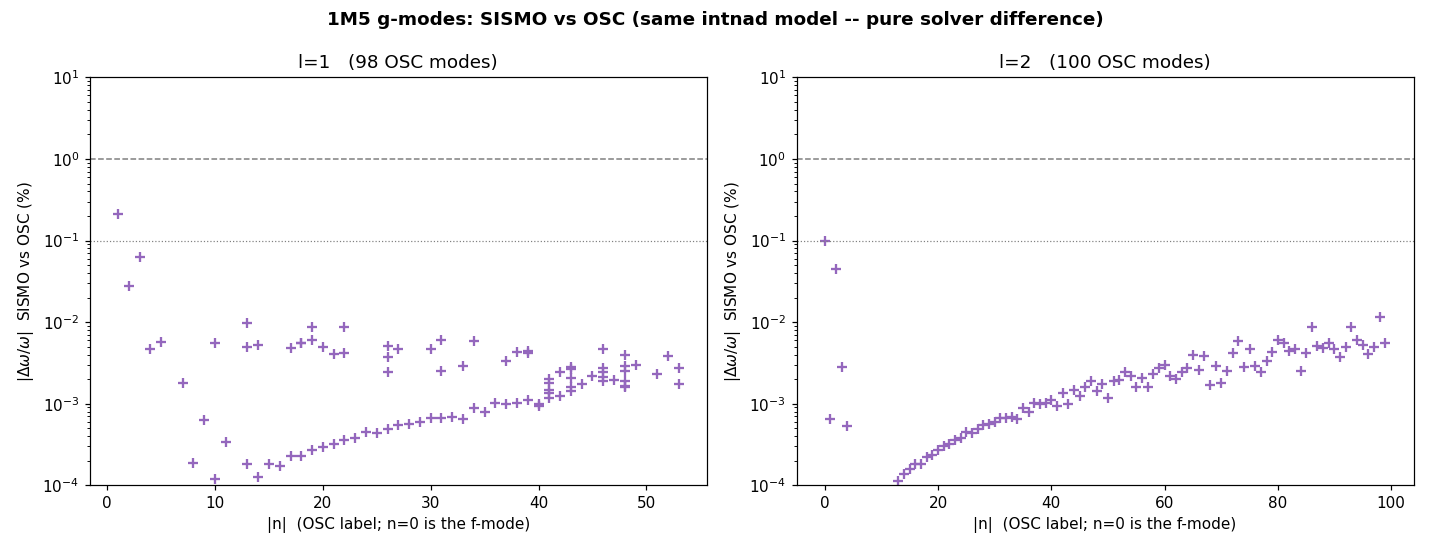
\includegraphics[width=\hsize]{FIGS/compare_core2_osc.png}
\caption{Relative frequency differences between the present split-Poisson
code and OSC, computed using the same $24,992$-point stellar model, as a
function of the radial-order label reported by OSC. The fundamental mode is
labelled $n=0$. The left and right panels show the results for $\ell=1$ and
$\ell=2$, respectively. The smooth increase towards high radial order
reflects the difference between the two discretisation schemes. All modes,
including the fundamental mode, agree to better than
$2.1\times10^{-3}$.}
\label{fig:osc}
\end{figure*}

\begin{figure*}
\centering
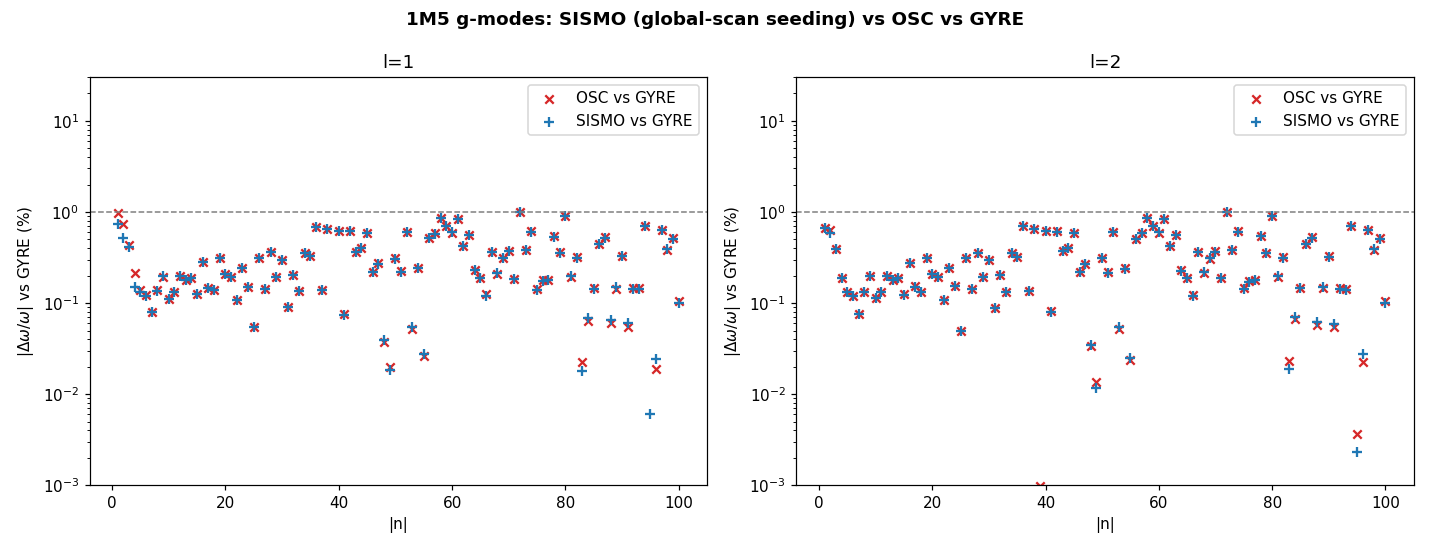
\includegraphics[width=\hsize]{FIGS/compare_core2_gyre.png}
\caption{Relative frequency differences with respect to GYRE for $\ell=1$
(left) and $\ell=2$ (right). Crosses show the OSC--GYRE comparison, while
plus signs show the differences between the present code and GYRE. The two
sets of differences follow the same characteristic level of approximately
$2\times10^{-3}$, which is attributed primarily to the interpolation and
remeshing of the equilibrium model.}
\label{fig:gyre}
\end{figure*}
Table~\ref{tab:accuracy} and Figs.~\ref{fig:osc}--\ref{fig:gyre} summarise
the accuracy of the computed frequencies. Three main results emerge from
these comparisons.
\paragraph{Differences between the solvers follow a smooth discretisation
trend.}When the present code and OSC are applied to the same stellar model, the
frequency differences remain small and vary smoothly with radial order. For
$\ell=2$, they increase from approximately $10^{-6}$ around
$|n|\simeq15$ to approximately $10^{-4}$ at $|n|=100$
(Fig.~\ref{fig:osc}). This trend is consistent with the accumulated
difference between the exponentially fitted staggered discretisation used
here and the finite-difference scheme applied by OSC on mode-dependent
refined grids. As expected for methods of comparable order, the discrepancy
increases with the radial wavenumber of the mode. The absence of isolated outliers is also noteworthy. All modes follow the
same continuous trend, indicating that the Sturm scan identifies the
spectrum consistently and that the subsequent fixed-point refinement
converges uniformly across the selected range of radial orders.

\paragraph{The dipole and quadrupole branches reach comparable accuracy.}

With the first-integral closure applied to the Poisson problem, the
$\ell=1$ frequency differences exhibit essentially the same behaviour as
those obtained for $\ell=2$. The largest dipole discrepancy,
$2.1\times10^{-3}$, occurs for the mode immediately adjacent to the
fundamental mode. This mode also has the largest Cowling shift in the
benchmark set, approximately $5.5\%$. For this least favourable mode, the remaining discrepancy corresponds to
approximately $4\%$ of the Cowling shift, implying that the global closure
removes about $96\%$ of the source-related error. By contrast, when the
homogeneous amplitude of the potential is determined solely from the surface
matching condition, the dipole errors follow an envelope approximately equal
to $1.3$ times the local Cowling shift. This envelope decreases roughly as
$n^{-2.4}$ but reaches several percent for the lowest-order modes. The use
of Takata's first integral is therefore essential for obtaining comparable
accuracy for the dipole and quadrupole branches.

\paragraph{The fundamental mode is located by the same counting procedure.}

The fundamental mode requires no dedicated search strategy. In the present
formulation, it is identified as the next change in the corrected Sturm count
above the g-mode sequence and is subsequently refined using the same
fixed-point iteration as all other modes. Its frequency agrees with the OSC
value to within $1.4\times10^{-3}$. This represents an improvement over the response-based scans used in the
first implementation of the code, which were unable to identify the
fundamental mode reliably because a probe constructed from a g-mode-like
eigenfunction produces little resonant response at the f-mode frequency.



\subsection{Anatomy of the error along the branch}

The comparison against the coupled solver on the same model cleanly separates
the three error sources of the method:
\begin{itemize}
\item \emph{Discretisation} dominates for $|n|\gtrsim15$: the smooth curve of
  Fig.~\ref{fig:osc}, growing with wavenumber, identical in shape for both
  degrees.  It is controlled by the grid (here, the native model grid) and
  would respond to Richardson extrapolation or higher-order fitting if
  smaller residuals were required.
\item \emph{Residual dipole source error} dominates the lowest dipole orders:
  the $\lesssim2\times10^{-3}$ remnants of the $\simeq5\%$ Cowling shifts,
  i.e.\ the part of the potential not captured by the least-squares first
  integral with the converged (but not exact) mechanical source.
\item \emph{Fixed-point truncation} is monitored explicitly. With the release
  tolerance, modes that satisfy the raw Newton criterion stop at an effective
  relative correction of $10^{-7}$; a
  bounded residual cycle instead returns its smallest-correction iterate.
  The direct OSC comparison below includes both cases.
\end{itemize}

%=============================================================================
\subsection{Computational cost}
\label{sec:performance}
\begin{table} \caption{Wall-clock and CPU times for the complete benchmark ($\ell=1,2$, $|n|=1\dots100$) on one 18-core workstation. GYRE runs on its own $1131$-point input model with internal remeshing and is listed for context; OSC, the first-generation code, and the present code all process the identical $24\,992$-point model.} \label{tab:timing} \centering \begin{tabular}{lccc} \hline\hline Code & wall & CPU & modes \\ \hline GYRE 8.1 (own grid) & $9.4$\,s & $71$\,s & 200 \\ OSC (scang, {\tt oscQI}=2) & $72.5$\,s & $1095$\,s & 202 \\ First-generation split code & $72.7$\,s & $905$\,s & 204 \\ Present code & $1.7$\,s & $28$\,s & 216 \\ \hline\hline \end{tabular} \end{table}
The timings are summarised in Table~\ref{tab:timing}. Relative to the coupled
reference calculation performed on the same stellar model, the approximately
fortyfold reduction in wall-clock time results from three main
properties of the numerical formulation.
\\~\\First, each evaluation of the mechanical operator requires only the assembly
and factorisation of a scalar tridiagonal matrix. Both operations scale as
$\mathcal{O}(N)$ and have a small numerical prefactor, in contrast to the
factorisation of the $4\times4$ block-banded system used in the fully coupled
formulation. This low cost makes the direct Sturm scan practical: the complete
scan, bisection, and refinement workflow finishes in about $1.7$\,s.
\\~\\Second, the Sturm scan eliminates the need for mode-dependent initial
frequency estimates and associated seeding procedures. The matrix
factorisations at the trial frequencies, the bisections of the identified
eigenvalue intervals, and the subsequent mode refinements are mutually
independent. These operations can therefore be distributed directly across
threads with little communication overhead. For the complete benchmark, the
wall-clock time decreases from $23.6$\,s in serial execution to $1.7$\,s
when using 18 threads. Third, the calculation is performed on the original model grid throughout.
No multigrid procedure, mode-dependent mesh refinement, or intermediate
remeshing is required. In addition to reducing the computational overhead,
this avoids introducing interpolation errors associated with transferring
the equilibrium structure or the eigenfunctions between different grids. The memory requirement consists of a small number of
$\mathcal{O}(N)$ work arrays for each thread. The complete implementation
contains approximately 2500 lines of source code.


%=============================================================================
\section{Summary and outlook}
\label{sec:conclusion}

We have shown that a fully inhomogeneous (split) treatment of the
gravitational potential reproduces coupled adiabatic oscillation
calculations at the level of the discretisation error -- median
$2\times10^{-5}$, maximum $2\times10^{-3}$ relative against OSC on the
identical model over the complete $\ell=1,2$, $|n|\le100$ spectrum including
the fundamental -- at roughly one fortieth of the wall-clock cost.  The three
ingredients that make this possible are:

\begin{enumerate}
\item an exact reduction of the mechanical pair to one scalar second-order
  equation, discretised by a cell-wise exponentially fitted box scheme whose
  tridiagonal matrix has positive off-diagonal products;
\item mode location by a pole-corrected Sturm parity scan of that matrix,
  which locates gravity, fundamental, and pressure modes without mode-by-mode
  asymptotic seeding, provided that the period grid resolves adjacent modes;
\item for the dipole, a parameter-free closure of the independent Poisson
  problem by least-squares enforcement of Takata's first integral, replacing
  the surface matching condition whose globally propagated amplitude error
  was identified as the origin of the classical split-scheme dipole bias.
\end{enumerate}

The eigenvalue operator never contains the potential; the architecture is
therefore ready for the programme that motivated it: the perturbative and
non-perturbative introduction of rotational (Coriolis) source terms computed
from the current eigenfunction, using the same frozen-source iteration, the
same Sturm location on the non-rotating operator, and -- for the dipole --
the rotating generalisation of the first integral.

\begin{acknowledgements}
\dots
\end{acknowledgements}

\begin{thebibliography}{}

\bibitem[Fellay \& Dupret(2025)]{Fellay2025}
Fellay, L., \& Dupret, M.-A. 2025, A\&A, 694, A51

\bibitem[Fellay et al.(2026)]{Fellay2026}
Fellay, L., Dupret, M.-A., \& Ko\l{}aczek-Szyma\'nski, P. A. 2026,
A\&A, 708, A109

\bibitem[Christensen-Dalsgaard(2008)]{jcd2008}
Christensen-Dalsgaard, J. 2008, Ap\&SS, 316, 113

\bibitem[Christensen-Dalsgaard \& Mullan(1994)]{jcd_mullan1994}
Christensen-Dalsgaard, J., \& Mullan, D. J. 1994, MNRAS, 270, 921

\bibitem[Paxton et al.(2011)]{paxton2011}
Paxton, B., Bildsten, L., Dotter, A., et al. 2011, ApJS, 192, 3

\bibitem[Scuflaire et al.(2008)]{scuflaire2008}
Scuflaire, R., Montalb\'an, J., Th\'eado, S., et al. 2008, Ap\&SS, 316, 149

\bibitem[Takata(2005)]{takata2005}
Takata, M. 2005, PASJ, 57, 375

\bibitem[Takata(2006)]{takata2006}
Takata, M. 2006, PASJ, 58, 893

\bibitem[Townsend \& Teitler(2013)]{townsend2013}
Townsend, R. H. D., \& Teitler, S. A. 2013, MNRAS, 435, 3406

\bibitem[Unno et al.(1989)]{unno1989}
Unno, W., Osaki, Y., Ando, H., Saio, H., \& Shibahashi, H. 1989, Nonradial
Oscillations of Stars, 2nd edn.\ (Tokyo: University of Tokyo Press)

\bibitem[Wilkinson(1965)]{wilkinson1965}
Wilkinson, J. H. 1965, The Algebraic Eigenvalue Problem (Oxford: Clarendon
Press)

\end{thebibliography}

\end{document}
